\documentclass[11pt,a4paper]{article}

\usepackage{alltt}
\usepackage[utf8]{inputenc}
\usepackage[english]{babel}
\usepackage{amsmath}
\usepackage{amsfonts}
\usepackage{amssymb}
\usepackage{indentfirst}
\usepackage{setspace}
\usepackage[pdftex]{graphicx}
\usepackage{caption}
\usepackage{subcaption}
\usepackage{textcomp}
\usepackage{array}
\usepackage{listings}
\usepackage{color}
\usepackage{tikz} % для создания иллюстраций

\newcommand{\infers}{\,\to\,}
\newcommand{\tinfers}{\;\Rightarrow\;}

\voffset = -118pt
\textheight = 820pt
\hoffset = -100pt
\textwidth = 550pt
\newcommand{\htext}{0.46\textwidth}
\newcommand{\hstext}{0.45\textwidth}

\newcommand{\mat}[1]{\overline{#1}}
\newcommand{\framed}[1]{\tikz[baseline=(char.base)]{\node[shape=rectangle,draw,inner sep=4pt] (char) {#1};}}

%opening
\title{}
\author{}

\begin{document}

\maketitle

Note! Copying .xyz files in Meson didn't work for me, so I had to copy them to build directory by hand.

\section*{Velocity-Verlet integrator}

Lennard-Jones potential - Pauli repulsion and London dispersion (attraction) (REF)

Velocity-Verlet integration (REF)


\[ \dot{\mat{v}}_i(t) = \cfrac{\mat{f}_i(t)}{m_i} \]
\[ \dot{\mat{r}}_i(t) = \mat{v}_i(t) \]

The movement is approximated by assuming constant force and making small time steps. We take Newton's law and definition of velocity, using Taylor formula, we get the approximation equations. (REF Lec 2)

Allen, Michael P., and Dominic J. Tildesley, Computer Simulation of Liquids, 2nd edn (Oxford, 2017; online edn, Oxford Academic, 23 Nov. 2017)


Predictor step:
\[
v_i(t + \Delta t/2) = v_i(t) + \cfrac{1}{2m_i} f_i(t) \Delta t
\]
\[ r_i(t+\Delta t) = r_i(t) + v_i(t+ \Delta t/2) \Delta t \]

Corrector step:
\[ v_i(t+\Delta t) = v_i(t+\Delta t/2) + \cfrac{1}{2m_i}f_i(t+\Delta t) \Delta t \]

{\bf Implementation} --- src/atoms.h, src/verlet.cpp, src/verlet.h, tests/test\_verlet.cpp

\section*{Lec 2}


\section*{Milestone 4. Lennard Jones potential with direct summation}

How to compute forces from energy. By definition of pair potential:
\[
E_{pot} = \sum_{i<j} V(r_{ij})
\]

Lennard-Jones potential is sum of Pauli Repulsion (repulsive force) and London Dispersion (attractive force). These interactions act even on uncharged atoms.

(REF Lec 3 Müser, M. H., Sukhomlinov, S. V., and Pastewka, L. (2022). Interatomic potentials: achievements and challenges. Advances in Physics: X, 8(1). https://doi.org/10.1080/23746149.2022.2093129)

\[
V_{ij}(r) = 4\epsilon \left( \Bigl(\cfrac{\sigma}{r}\Bigr)^{12} - \Bigl(\cfrac{\sigma}{r}\Bigr)^{6} \right)
\]

By definition of energy, force is the derivative of energy by position.
\[
\mat{f}_k = \left( \begin{aligned}
	& - \partial E / \partial x_k \\
	& - \partial E / \partial y_k \\
	& - \partial E / \partial z_k \\
\end{aligned} \right) = \sum_i \cfrac{\partial V}{\partial r_{ik}} {\hat r_{ik}} \text{\ (unit vector)}
\]

Let's compute for one of the dimensions.
\[
\cfrac{\partial V_{ij}}{\partial x_k} = \text{(chain rule by vector length)} \cfrac{\partial V_{ij}}{\partial r_{ij}} \cfrac{\partial r_{ij}}{\partial x_k}
\]

\[ \cfrac{\partial r_{ij}}{\partial x_k} = \cfrac{\partial \sqrt{(x_j-x_i)^2 + \ldots}}{\partial x_k} = (*) \]
Remember: \( (\sqrt{u})' = \cfrac{1}{2\sqrt{u}} u' \)

\[
(*) = \cfrac{1}{2r_{ij}} \cfrac{(x_j-x_i)^2+\ldots}{\partial x_k} = \cfrac{1}{r_{ij}} \cdot (x_j-x_i) \cdot \Bigl(\cfrac{\partial x_j}{\partial x_k} - \cfrac{\partial x_i}{\partial x_k}\Bigr)
\]
Here is a pair of atoms $i$ and $j$. We want the force for atom $k$. If \(k\neq i\) and \(k\neq j\), the expression is 0.

\[
(*) = \left( \begin{aligned}
	& (x_j - x_i) (\delta_{jk} - \delta_{ik}) / r_{ij} \\
	& (y_j - y_i) (\delta_{ik} - \delta_{jk}) / r_{ij} \\
	& (z_j - z_i) (\delta_{ik} - \delta_{jk}) / r_{ij} \\
\end{aligned} \right) 
\]

\[
k=j \infers (x_k-x_i)(1-0)/r_{ik},\ (*) = {\hat r_{ik}}
\]
\[
k=i \infers (x_j-x_k)(0-1)/r_{kj},\ (*) = {\hat r_{jk}}
\]

When we take the derivative of energy, only the pairs, where one of the atoms is \(k\), are left. The derivative is exactly the same for \(V_{ij}\) and \(V_{ji}\).

{\centering\framed{ \( \mat{f}_k = - \sum_i \cfrac{\partial V}{\partial r} {\hat r_{ik}} \) }\\}

Last piece in the puzzle is derivative of potential by distance.

\[
\cfrac{\partial V}{\partial r} = 4\epsilon (\sigma^{12} (-12) r^{-13} - \sigma^6\cdot 6\cdot r^{-7})
\]

\section*{First molecular dynamics simulation}
In the first simulation, we don't care about physical units, and just set \( m=1, \sigma=1, \epsilon=1 \). Simulation duration is \( 100 \sqrt{m\sigma^2 / \epsilon} \), the atom positions are saved each \( 1 \sqrt{m\sigma^2 / \epsilon} \).  

Experimentally choosing the time step (multiplied by \( \sqrt{m\sigma^2 / \epsilon} \)): 0.001 --- OVITO visualization shows that most of atoms evaporate and fly into infinity; 0.00001 --- most atoms stay together, while some still evaporate. We can also detect evaporation if potential energy increases and kinetic energy doesn't change. The total energy was plotted for different time steps in Fig.~\ref{fig:first_simulation}.

{\bf Implementation} --- src/lj\_direct\_summation.cpp, src/lj\_direct\_summation.h, tests/test\_lj\_direct\_summation.cpp src/xyz.cpp, src/xyz.h, tests/test\_verlet.cpp, milestones/04/main.cpp

\begin{figure*}[htb]
	\centering
	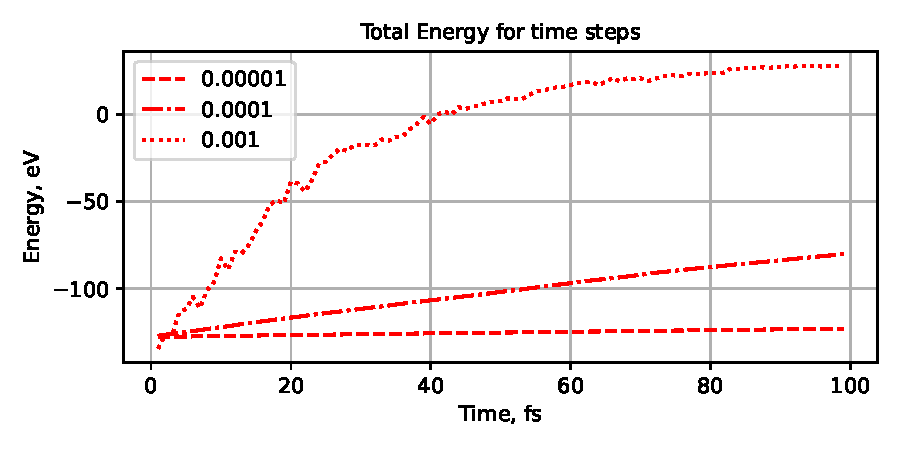
\includegraphics[width=.7\linewidth]{img/fig.pdf}
	\caption{Total energy behaviour is better with very small time step.}
	\label{fig:first_simulation}
\end{figure*}

\begin{figure*}[htb]
	\centering
	\begin{minipage}{.3\textwidth}
		\centering
		\resizebox{\columnwidth}{!}{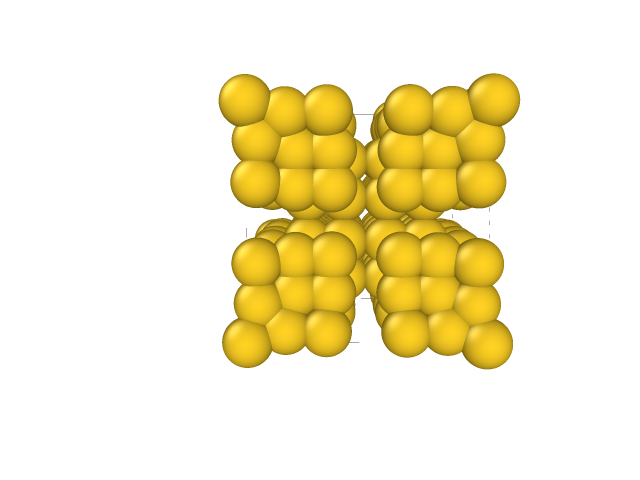
\includegraphics[trim={1.8cm 1.8cm 2.2cm 1.8cm},clip]{img/sim1.png}}
	\end{minipage}\hfill
	\begin{minipage}{.3\textwidth}
		\centering
		\resizebox{\columnwidth}{!}{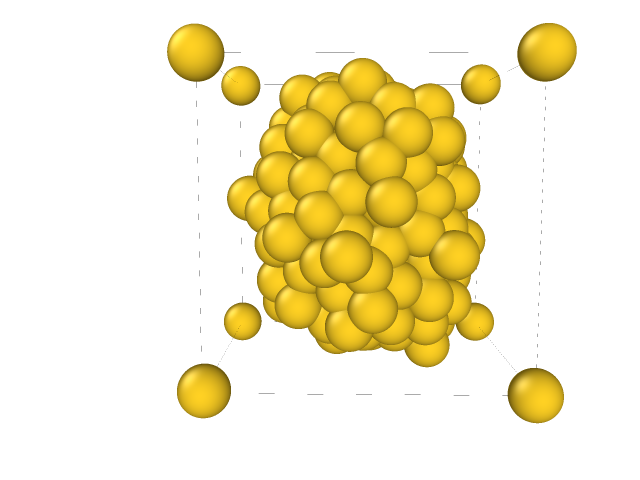
\includegraphics[trim={1.8cm 1.8cm 2.2cm 1cm},clip]{img/sim2.png}}
	\end{minipage}\hfill
	\begin{minipage}{.3\textwidth}
		\centering
		\resizebox{\columnwidth}{!}{
			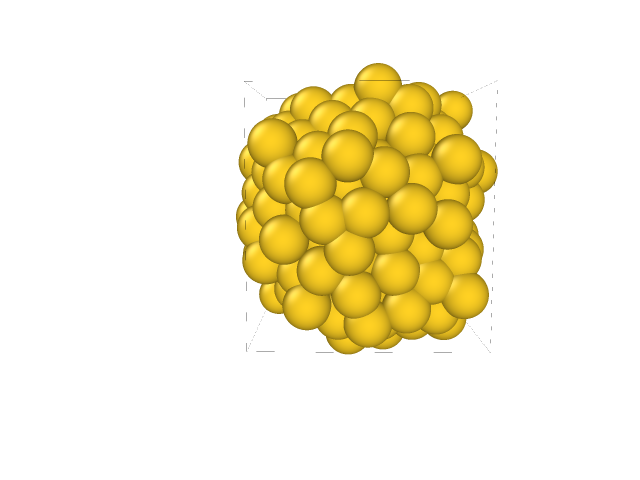
\includegraphics[trim={1.8cm 1.8cm 2.2cm 1cm},clip]{img/sim3.png}}
	\end{minipage}
	\caption{OVITO visualization. Without thermostat, atoms vaporize even with the smallest time step.}
	\label{fig:first_simulation_ovito}
\end{figure*}




\section*{Berendsen thermostat}
As the molecular dynamics system evolves, potential energy decreases and kinetic energy increases, therefore we connect the system to a heat bath of constant temperature, which stabilizes the simulation. (REF)

To decrease the temperature, we scale the velocities of atoms by a factor

\[ v' = \lambda v,\ \lambda = \sqrt{1 + \left(\cfrac{T_0}{T}-1 \right) \cfrac{\Delta t}{\tau} }  \]
\[ E_k = \cfrac{1}{2} \sum_i m_i v_i^2 = \cfrac{3}{2} N K_b T \infers T = \cfrac{2}{3} \cfrac{E_k}{K_b N} \]

\(T_0\) is target temperature, \(\Delta t = 0.0001 \sqrt{m\sigma^2 / \epsilon} \) from the first simulation, \( \tau \) is relaxation time of the thermostat and should be much larger than the time step.

I create a cube of atoms of width 4 for this experiment

Choosing target temperature: 0.05 --- visualization shows that the atoms are pushed apart into infinity in small groups; 0.005 --- no vaporization.

Choosing Berendsen relaxation time: for whole simulation, \(1000\delta t\) is required to keep the atoms from evaporating; initial strong relaxation doesn't make a difference.

Time: n=2, t=0.5; n=3, t=6; n=4, t=30.

{\bf Implementation} --- src/lj\_direct\_summation.cpp, src/lj\_direct\_summation.h, tests/test\_lj\_direct\_summation.cpp src/xyz.cpp, src/xyz.h, tests/test\_verlet.cpp, milestones/05/main.cpp

\section*{Milestone 6. Neighbor list}

Cutoff radius is \( 3 \sigma \) to allow speedup.

\end{document}
